%\documentclass[11pt]{article}

\documentclass[addpoints,12pt]{exam}

\usepackage[margin=2.5cm]{geometry}
\usepackage{graphicx}
\usepackage{listings}
\usepackage{xpatch}
\usepackage{color}
\usepackage{amsmath}
\usepackage[utf8]{inputenc}

\makeatletter
\xpretocmd{\item@points@pageinfo}{\normalfont}{}{}
\xapptocmd{\item@points@pageinfo}{\bfseries}{}{}
\makeatother

\begin{document}
	\begin{center}
		\LARGE\scshape{Fluorescencia}
		
		\vspace{1cm}
		\large\scshape{Juan Barbosa - 201325901}
	\end{center}

	La microscop\'ia de fluorescencia es una importánte técnica de microscop\'ia ya que permite observar objetos diminutos con gran magnificación y resolución. En el caso de la fluorescencia no se usa luz transmitida sino luz reflejada (o luz emitida por la muestra).
	
	\begin{figure}[h]
		\centering
		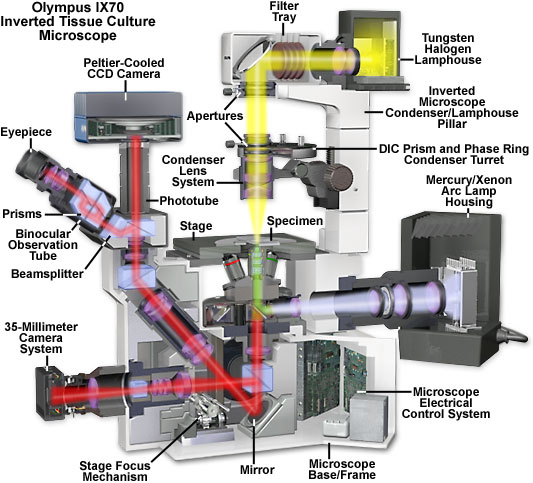
\includegraphics[width = 0.5\linewidth]{lightpaths.jpg}
	\end{figure}
	
	El esquema general del camino óptico de un microscópio de fluorescencia se muestra en la figura anterior. Un haz de luz se hace insidir sobre un filtro pasa bandas, el cual se conoce como el filtro de excitación. Posteriormente el haz pasa por el espéjo dicrócico, el cual refleja y transmite longitudes de onda específicas. Parte de la luz va en dirección en direcci\'on a la muestra, donde la luz incidente excita los fluor\'oforos en la muestra. Estos pueden ser propios de la muestra (autofluorescencia) o tintes agregados a la misma. La luz emitida pasa atrav\'es del dicr\'oico hasta alcanzar el filtro de emisi\'on, el cu\'al permite limitar la cantidad de fluor\'oforos detectados. Finalmente la luz llega al ocular, o a una c\'amara CCD.
	
	\begin{questions}
		{\question Qu\'e es un filtro de densidad neutra}
		
		Los filtros de densidad neutra son filtros que reducen la intensidad de la luz de forma homog\'enea para todas las longitudes de onda de la luz incidente.
		
		{\question Para qu\'e la apertura num\'erica est\'a optimizada para la c\'amara si se considera un factor de muestreo de 3?}
		
		En el datasheet se especifica que el tama\~no de los pixeles es de 6.45 x 6.45 $\mu$m. En una ccd la luz se proyecta sobre el plano de los pixeles. Existen dos posibles efectos en la proyecci\'on, por un lado es posible que demasiados pixeles contengan al mismo punto de Airy, lo cual implica informaci\'on redundante. En el caso opuesto cada pixel tendr\'a la informaci\'on de varios c\'irculos de Airy, lo cual no permite resolver los detalles.
		
		El tama\~no de la proyecci\'on ser\'a entonces:
		\begin{equation}
			P = \left(\dfrac{1.22\lambda}{2NA}\right)M \qquad \text{M: magnificaci\'on, NA: apertura num\'erica}
		\end{equation}
		
		La idea es que el tama\~no de la proyecci\'on sea de 3 pixeles:
		\begin{equation}
			\left(\dfrac{M}{NA}\right) \approx \dfrac{3(6.45)}{0.244} \approx 60 \qquad \text{con $\lambda = 500$ nm}
		\end{equation}
		
		{\question Qu\'e campo de visi\'on tienen los objetivos de 20x y 40x con la c\'amara dada?}
		Suponiendo aperturas num\'ericas de 1.3x 
	\end{questions}
\end{document}
